% !TeX root = responsiveness_tr
% ================================================================
\section{Approximations}\label{prresp_approx}

The per-ACK EWMA is not intended to mimic a per-RTT EWMA. Otherwise, the per-ACK
EWMA would have to reach the same value by the end of the round, irrespective of
whether markings arrived early or late in the round.
It is more important for the EWMA to quickly accumulate any markings early in
the round than it is to ensure that the EWMA reaches precisely the same value by
the end of the round. 

Neither is it important that a per-ACK EWMA decays at precisely the same rate as
a per-round EWMA (assuming they both use the same gain). The gain is not
precisely chosen, so if a per-ACK EWMA decays somewhat more slowly, it is
unlikely to be critical to performance (if so, a higher gain value can be
configured).

However, it \emph{is} important that a per-ACK EWMA decays at about the same
rate however many ACKs there are per round, although the decay rate does not
have to be precisely the same.

The per-ACK approach uses the approximation that one reduction with gain \(1/G\)
is roughly equivalent to \(n\) repeated reductions with \(1/n\) of the gain.
Specifically, that \((1 - 1/nG)^n \approx 1 - 1/G\).

\begin{align*}
(1 - 1/nG)^n &=       1 + \frac{n}{-nG} + \frac{n(n-1)}{2(-nG)^2} + \ldots \\
             &=       1 - \frac{1}{G} + O\left(\frac{1}{G^2}\right)\\
             &\approx 1 - \frac{1}{G}
\end{align*}

To quantify the error, we define the effective gain
(\(1/G^\prime\)) as the per-RTT gain that would give an equivalent reduction to
multiple smaller per-ACK reductions using the original gain (\(1/G\)).
Numerically, we find that \(G^\prime \approx G + 1/2\) (see \autoref{fig:per-ack-approx}).

\begin{figure}[h]
	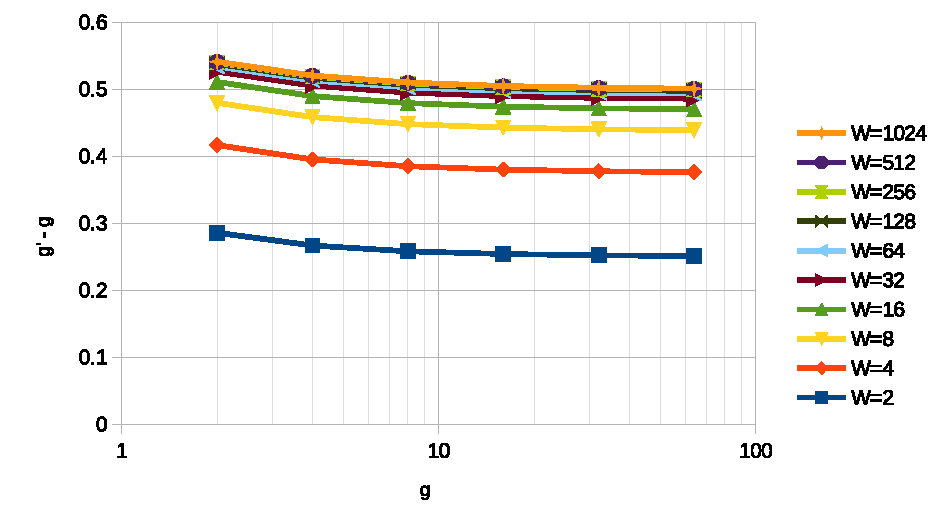
\includegraphics[width=\linewidth]{per-ack-approx}
	\caption{Difference between gain used for multiple per-ACK reductions, \(G^\prime\), and the gain of one equivalent reduction, \(G\).}
	\label{fig:per-ack-approx}
\end{figure}

For instance, multiple reductions with \(G\approx15.5\) are roughly equivalent to one
reduction with \(G^\prime=16\).

This can be explained because most of the error comes from omission of the
\(O(1/G^2)\) term. So we set
\begin{align*}
1-\frac{1}{G^\prime} &\approx 1 - \frac{1}{G} + \frac{(n-1)}{2nG^2},
\intertext{which, in the worst case of large \(n\), reduces to}
G^\prime &\approx \frac{2G^2}{(2G-1)}.
\intertext{Then the difference between the reciprocals of the effective and
	actual gains is}
G^\prime - G &\approx \frac{G}{(2G-1)}
\end{align*}
Other than for low values of \(G\) this difference is indeed roughly \(1/2\). 

The worst-case error occurs when \(G\) is small and \(W\) is large. Multiple reductions using any high value of \(W\) and the lowest practical value of \(G (=2)\)
would be equivalent to a single reduction using \(G^\prime\approx2.54\) (i.e.\
the error in this worst-case is about 0.54).
